\section{Setup and Experimental Apparatus }
\label{sec:setup}

We performed measurements of SiPM properties in the laboratory at Caltech using
signals from a class 3R PiLas laser which produces light at a wavelength of
$407$~nm. Beam measurements were performed at the H4 beam-line of the CERN
North-Area test-beam facility, which provides secondary beams of energies
ranging between $20$~GeV and $400$~GeV. The beams are composed of a mixture of
electrons and pions. The electron fraction in the beam is typically around 75\%.

The data acquisition (DAQ) system is based on a CAEN V1742 switched capacitor
digitizer~\cite{DRS4}, whose electronic time resolution has been measured to be
$4$~ps. Data readout for the laser-based measurements are triggered by an
external digital trigger signal, while at the H4 beamline readout is triggered
by a signal in a photomultiplier tube coupled to a
$X$~$\mathrm{cm}$~$\times$~$X$~$\mathrm{cm}$ plastic scintillator. A
micro-channel plate photo-multiplier (MCP-PMT) detector is used to provide a
very precise reference time-stamp in order to measure the time resolution of the 
SiPM signals.

\subsection{Setup for Laser-based SiPM Timing Measurements}

SiPMs are mounted on a printed circuit board (PCB) with a clipping capacitance
circuit shown in Figure~\ref{fig:Circuit}. The is mechanically attached to an
optical breadboard enclosed within a box lined with copper foil for RF
shielding. The laser is injected via a light-guide fiber mounted on an optical
holder. The laser beam is immediately split by a refractive mirror and half of
the light is directed straight into the MCP-PMT while the other half of the
light is directed onto the SiPM under test. A photograph of the setup is shown
in Figure~\ref{fig:laserSetup}. The Photek-240 MCP-PMT is used as the reference
time detector whose time resolution has been measured to be below $7$~ps for
beam particles~\cite{MCPShowerMaxPaper}. To cover a large range of laser beam
intensity, neutral density (ND) filters with attenuation factor between X and Y
are placed between the mirror and the SiPMs under test.

%Figure: Diagram of detector elements
\begin{figure}[htbp] 
\centering
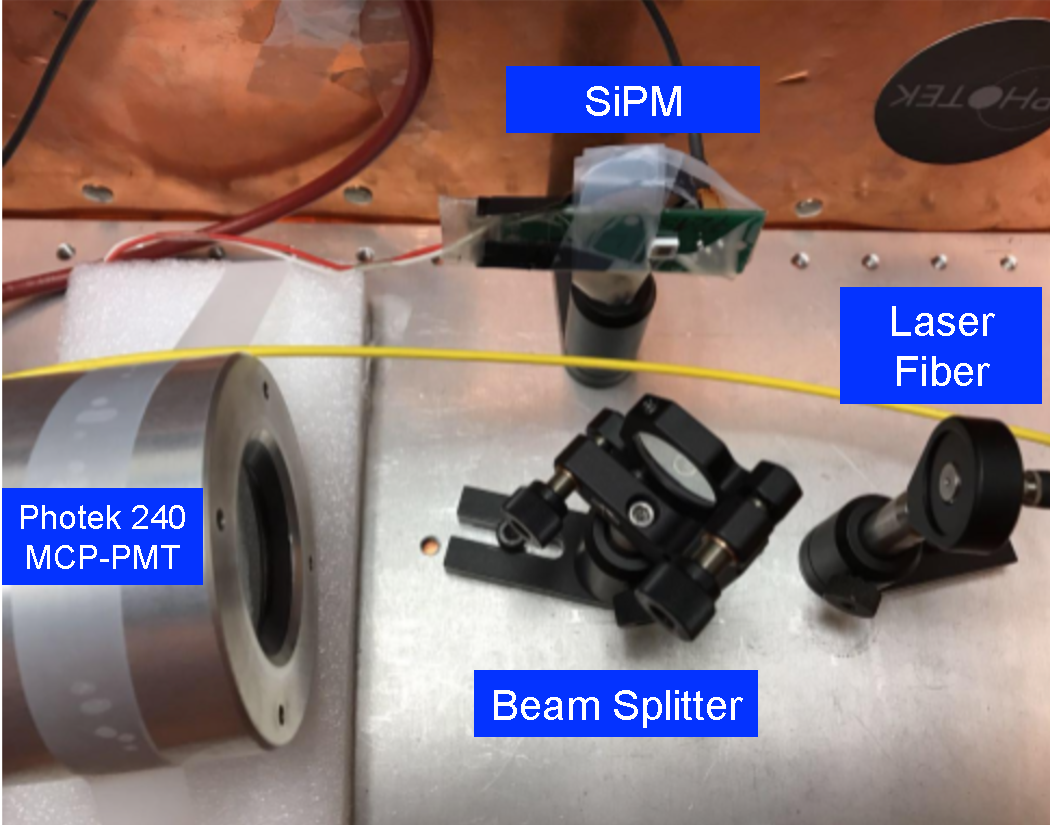
\includegraphics[width=0.49\textwidth]{figures/SiPMSetup1.pdf} 
\caption{Photograph of the Laser-based SiPM timing measurement setup.} 
\label{fig:laserSetup} 
\end{figure} 

\subsection{Setup for Timing Measurements of Scinittilators with SiPM readout.}

A Hamamatsu R3809U MCP-PMT~\cite{HamaMCPDataSheet} is used as the reference time 
detector whose time resolution has been measured to be about $15$~ps~\cite{Anderson:2015gha}.
%Did we do this?


\subsection{Timestamp Reconstruction}

The time-stamp for all signals is reconstructed by fitting the pulse waveform
with an appropriate functional form. For signal pulses from the MCP-PMTs, which
exhibit a very fast rise and decay, we fit a Gaussian function to a $1.5$~ns
window around the peak of the pulse and extract the time-stamp as the mean
parameter of the Gaussian function. For signal pulses from the SiPM sensors, we
fit a linear function to time sample points between $10\%$ and $60\%$ of the
pulse maximum and the time-stamp is assigned as the time at which the fitted
linear function rises to $30\%$ of the pulse maximum. More details of the
time-stamp reconstruction can be found in reference~\cite{Anderson:2015gha}.
